\documentclass[11pt,a4paper]{article}
\usepackage[T1]{fontenc}
\usepackage[utf8]{inputenc}
\usepackage{lmodern}
\usepackage{textcomp}
\usepackage[left=1.8cm,right=1.8cm,top=3.0cm,bottom=2.2cm,headheight=36pt,headsep=12pt]{geometry}
\usepackage{multicol}
\usepackage{xcolor}
\usepackage{fancyhdr}\usepackage{tikz}
\usepackage{graphicx}
\usepackage{array}
\usepackage{amsmath,amssymb}
\usepackage{setspace}
\usepackage{longtable}
\graphicspath{{../}}
\definecolor{ygreen}{RGB}{46,139,87}\definecolor{dgreen}{RGB}{28,90,56}
\renewcommand{\normalsize}{\fontsize{10.9}{13.4}\selectfont}
\renewcommand{\familydefault}{\rmdefault}
\setlength{\parindent}{0pt}
\setlength{\columnsep}{0.8cm}
\setlength{\columnseprule}{0.4pt}
\setlength{\multicolsep}{3pt plus 1pt minus 1pt}
\renewcommand{\textsubscript}[1]{\ensuremath{_{\text{\fontsize{8}{8}\selectfont #1}}}}
\renewcommand{\textsuperscript}[1]{\ensuremath{^{\text{\fontsize{8}{8}\selectfont #1}}}}
\newcommand{\qn}[1]{\textbf{\fontsize{11.5}{13}\selectfont #1}}
\newcommand{\qsep}{\par\vspace{13pt}}
\newcommand{\fwrule}{\par\vspace{5pt}\noindent\rule{\linewidth}{1.4pt}\par\vspace{7pt}}
\newsavebox{\fitb}
\newcommand{\fitbox}[1]{\sbox{\fitb}{#1}\ifdim\wd\fitb>\linewidth\resizebox{\linewidth}{!}{\usebox{\fitb}}\else\usebox{\fitb}\fi}
\newcommand{\diqqat}[1]{\par\smallskip\noindent\textbf{Diqqat!} #1\par\medskip}
\newcommand{\javob}{\par\nopagebreak[4]\smallskip\noindent\textbf{Javob:} \rule[-2pt]{7.5cm}{0.4pt}\par\smallskip\noindent\textbf{Diqqat!} Javobingizni javoblar varaqasiga ko`chirib yozing.\par\medskip}
\pagestyle{fancy}
\fancyhf{}
\renewcommand{\headrulewidth}{1.6pt}\renewcommand{\headrule}{{\color{ygreen}\hrule height 1.6pt width\headwidth}}
\newcommand{\hdrlogo}{
\begin{tikzpicture}[baseline=0pt]\fill[ygreen,rounded corners=3pt] (0,0) rectangle (0.95,0.95);\node[white,font=\fontsize{24}{26}\bfseries\selectfont] at (0.475,0.47){K};\node[anchor=west,font=\fontsize{16}{18}\bfseries\selectfont,text=dgreen] at (1.15,0.66){KIMYO};\node[anchor=west,font=\footnotesize\scshape,text=gray] at (1.15,0.2){Milliy sertifikat\ \ 2026};\end{tikzpicture}}
\newcommand{\hdrpill}[1]{\begin{tikzpicture}[baseline=0pt]\node[fill=ygreen,text=white,rounded corners=8pt,inner xsep=10pt,inner ysep=5pt,font=\fontsize{13}{15}\bfseries\selectfont] at (0,0.475){#1};\end{tikzpicture}}
\fancyhead[L]{\hdrlogo}
\fancyhead[R]{\hdrpill{7-variant}}

\fancyfoot[C]{\thepage}
\fancypagestyle{first}{\fancyhf{}\renewcommand{\headrulewidth}{1.6pt}\renewcommand{\headrule}{{\color{ygreen}\hrule height 1.6pt width\headwidth}}\fancyhead[L]{\hdrlogo}\fancyhead[R]{\hdrpill{7-variant}}\fancyfoot[C]{\thepage}}
\begin{document}
\normalsize
\thispagestyle{first}
\noindent\textit{Davriy jadvaldan foydalanish mumkin.}
\par\smallskip
\begin{multicols}{2}
\noindent\qn{1.} Rasmda tasvirlangan A elementi haqida qaysi fikr to`g`ri?
\begin{center}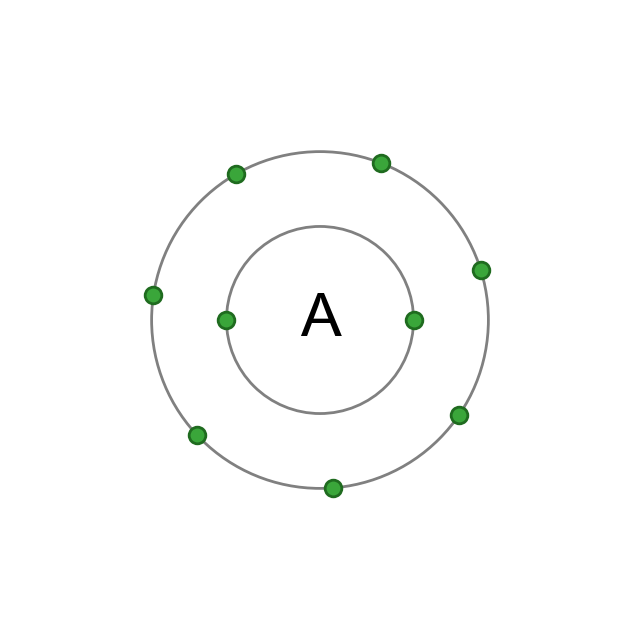
\includegraphics[width=0.86\linewidth]{rasmlar/gen/atom_9_16432.png}\end{center}
\noindent A)~\textsl{Metall, oksidi asosli xossali}\par
\noindent B)~\textsl{Metall, vodorodli birikma hosil qilmaydi}\par
\noindent C)~\textsl{Metallmas, oksidi kislotali xossali}\par
\noindent D)~\textsl{Inert gaz, birikmalar hosil qilmaydi}\par
\qsep
\noindent\qn{2.} VA guruh elementlarining vodorodli birikmalari qaynash haroratlari grafikda berilgan.
\begin{center}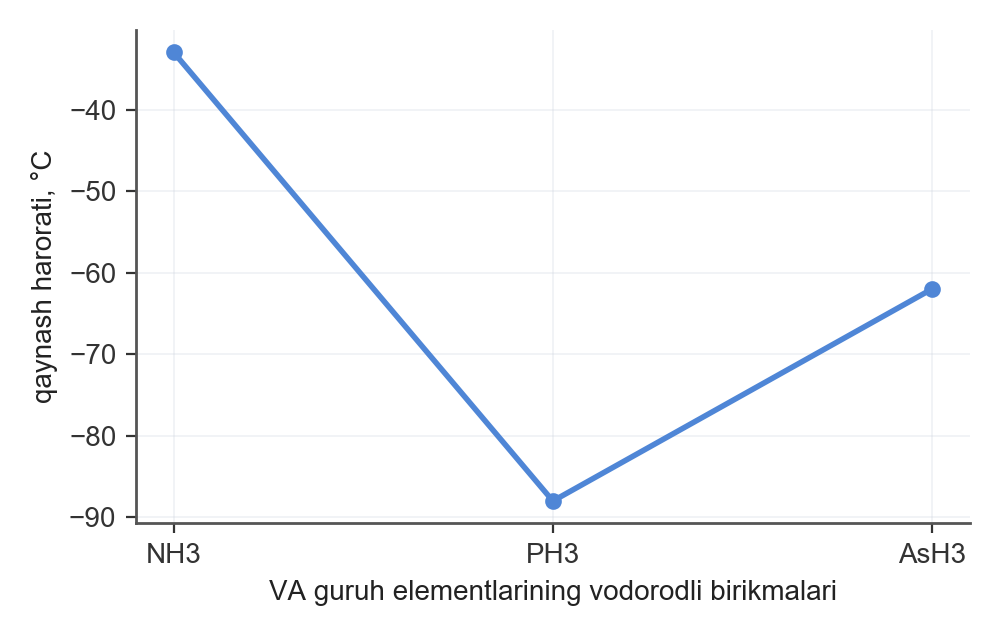
\includegraphics[width=0.86\linewidth]{rasmlar/gen/hy2_v07_0.png}\end{center}
NH\textsubscript{3} ning qaynash harorati yuqoriligining sababi nima?
\noindent A)~\textsl{Molekula massasi kattaligi}\par
\noindent B)~\textsl{Ion bog`lanish mavjudligi}\par
\noindent C)~\textsl{Kovalent bog` mustahkamligi}\par
\noindent D)~\textsl{Molekulalararo vodorod bog`lanish borligi}\par
\qsep
\noindent\qn{3.} Temir (\textit{Z} = 26) atomida nechta juftlashmagan elektron bor?

\noindent A)~\textsl{5} \hfill B)~\textsl{3} \hfill C)~\textsl{4} \hfill D)~\textsl{6}\par
\qsep
\noindent\qn{4.} KNO\textsubscript{3} ning suvli eritmasi inert elektrodlar bilan elektroliz qilinganda qaysi moddalar ajraladi?

\noindent\begin{tabular}{@{}p{0.47\linewidth}@{}p{0.47\linewidth}@{}}
A)~\textsl{H\textsubscript{2} va O\textsubscript{2}} & B)~\textsl{Zn, H\textsubscript{2} va O\textsubscript{2}} \\
C)~\textsl{Cu va Cl\textsubscript{2}} & D)~\textsl{H\textsubscript{2}, Cl\textsubscript{2} va NaOH} \\
\end{tabular}\par
\qsep
\noindent\qn{5.} pH = 2 bo`lgan HCl eritmasidan 180 ml va pH = 12 bo`lgan NaOH eritmasidan 220 ml aralashtirildi. Hosil bo`lgan eritmaning pH \textbf{ini aniqlang.}

\noindent A)~\textsl{12} \hfill B)~\textsl{11} \hfill C)~\textsl{10} \hfill D)~\textsl{7}\par
\qsep
\noindent\qn{6.} Mg va Al dan iborat 7,8 g qotishma mo`l xlorid kislotada eritildi. Ajralgan gaz kislorodda to`liq yondirildi. Reagent (xlorid kislota) eritmasining massa ulushi 10\% va zichligi 1,18 g/ml; u mo`l miqdorda olingan. Hosil bo`lgan suvning \textbf{massasini (g) hisoblang.}

\noindent A)~\textsl{7,2} \hfill B)~\textsl{9} \hfill C)~\textsl{3,6} \hfill D)~\textsl{14,4}\par
\qsep
\noindent\qn{7.} NiSO\textsubscript{4} tuzining kristallogidratida suvning massa ulushi 41,1\% ni tashkil etadi. Kristallogidrat formulasidagi suv molekulalari \textbf{sonini (n) toping.}

\noindent A)~\textsl{8} \hfill B)~\textsl{6} \hfill C)~\textsl{12} \hfill D)~\textsl{7}\par
\qsep
\noindent\qn{8.} 238\_92 yadro ketma-ket 8 ta $\alpha$- va 6 ta $\beta$\textsuperscript{$-$}-yemirilishga uchradi. Hosil bo`lgan barqaror yadrodagi neytronlar \textbf{sonini toping.}

\noindent A)~\textsl{128} \hfill B)~\textsl{124} \hfill C)~\textsl{122} \hfill D)~\textsl{82}\par
\qsep
\noindent\qn{9.} H\textsubscript{2} + I\textsubscript{2} $\rightleftarrows$ 2HI reaksiyasi 2 l hajmli idishda o`tkazildi. Ma'lumotlar jadvalda berilgan:
\begin{center}
\renewcommand{\arraystretch}{1.15}
\fitbox{\begin{tabular}{|c|c|c|c|}\hline
\textbf{Modda} & \textbf{H\textsubscript{2}} & \textbf{I\textsubscript{2}} & \textbf{HI} \\ \hline
Boshlang`ich, mol & 4 & 6 & 0 \\ \hline
Muvozanatda, mol & --- & --- & 3 \\ \hline
\end{tabular}}
\end{center}
Muvozanat \textbf{konstantasini (K) hisoblang.}

\noindent A)~\textsl{0,8} \hfill B)~\textsl{1,6} \hfill C)~\textsl{0,4} \hfill D)~\textsl{1,25}\par
\qsep
\noindent\qn{10.} H\textsubscript{2} + I\textsubscript{2} $\rightleftarrows$ 2HI sistemasida boshlang`ich moddalarning har biridan 2 mol dan 2 l hajmli idishga solindi. Muvozanat qaror topganda reagentlarning har birining 3/5 qismi sarflangan bo`ldi. Muvozanat \textbf{konstantasini hisoblang.}

\noindent A)~\textsl{18} \hfill B)~\textsl{4,5} \hfill C)~\textsl{10} \hfill D)~\textsl{9}\par
\qsep
\noindent\qn{11.} 25 g CuSO\textsubscript{4}$\cdot$5H\textsubscript{2}O qizdirilganda massa 3,6 g ga kamaydi. Qoldiq 300 g suvda to`liq eritildi. Qizdirish 45 daqiqa davom etdi. Hosil bo`lgan eritmadagi CuSO\textsubscript{4} ning massa \textbf{ulushini (\%) aniqlang.}

\noindent A)~\textsl{4,92} \hfill B)~\textsl{4,98} \hfill C)~\textsl{5,33} \hfill D)~\textsl{9,96}\par
\qsep
\noindent\qn{12.} Reaksiya tezligining haroratga bog`liqligi jadvalda berilgan:
\begin{center}
\renewcommand{\arraystretch}{1.15}
\fitbox{\begin{tabular}{|c|c|c|c|}\hline
\textbf{T, \textdegree{}C} & \textbf{20} & \textbf{30} & \textbf{40} \\ \hline
v, mol/(l$\cdot$s) & 1 & 2 & 4 \\ \hline
\end{tabular}}
\end{center}
Jadvaldan foydalanib, shu reaksiyaning 50 \textdegree{}C dagi tezligini (mol/(l$\cdot$s)) \textbf{aniqlang.}

\noindent A)~\textsl{4} \hfill B)~\textsl{16} \hfill C)~\textsl{8} \hfill D)~\textsl{6}\par
\qsep
\noindent\qn{13.} 2NO + O\textsubscript{2} $\to$ 2NO\textsubscript{2} reaksiyasi (v = k$\cdot$[NO]\textsuperscript{2}$\cdot$[O\textsubscript{2}]) harorati 20 \textdegree{}C ga oshirilib ($\gamma$ = 2), idish hajmi 3 marta kamaytirildi. Reaksiya tezligi necha marta ortadi?

\noindent A)~\textsl{216} \hfill B)~\textsl{54} \hfill C)~\textsl{4} \hfill D)~\textsl{108}\par
\qsep
\noindent\qn{14.} Ishqoriy metallar haqida qaysi fikrlar to`g`ri? 1) Natriy kerosin ostida saqlanadi; 2) Litiy eng yengil metall; 3) Ishqoriy metallar tabiatda erkin holda uchraydi; 4) Natriyning olinishi suyuqlanma NaCl elektrolizi bilan

\noindent A)~\textsl{1, 2, 4} \hfill B)~\textsl{2, 3} \hfill C)~\textsl{2, 3, 4} \hfill D)~\textsl{1, 3, 4}\par
\qsep
\noindent\qn{15.} D-metallar va ularning birikmalari haqida qaysi fikrlar to`g`ri? 1) Rux eritmada Fe\textsuperscript{2+} ni siqib chiqara olmaydi; 2) Zn(OH)\textsubscript{2} amfoter xossaga ega; 3) Mis suyultirilgan HCl bilan reaksiyaga kirishadi; 4) Mis nam havoda (CuOH)\textsubscript{2}CO\textsubscript{3} qoplamasi bilan qoplanadi

\noindent A)~\textsl{2, 3, 4} \hfill B)~\textsl{1, 4} \hfill C)~\textsl{3, 4} \hfill D)~\textsl{2, 4}\par
\qsep
\noindent\qn{16.} 0,5 mol CO\textsubscript{2} 0,62 mol NaOH eritmasidan o`tkazildi (reaksiya oxirigacha). Hosil bo`lgan tuzlar umumiy \textbf{massasini (g) aniqlang.}

\noindent A)~\textsl{53} \hfill B)~\textsl{44,8} \hfill C)~\textsl{42} \hfill D)~\textsl{89,5}\par
\qsep
\noindent\qn{17.} BaCO\textsubscript{3} va Na\textsubscript{2}CO\textsubscript{3} aralashmasi (101,5 g) mo`l xlorid kislota bilan ta'sirlashganda 15,68 l (n.sh.) gaz ajraldi. Sarflangan HCl \textbf{massasini (g) hisoblang.}

\noindent A)~\textsl{25,5} \hfill B)~\textsl{51,1} \hfill C)~\textsl{102,2} \hfill D)~\textsl{21,9}\par
\qsep
\noindent\qn{18.} FeCl\textsubscript{3} va NaCl aralashmasi tarkibida FeCl\textsubscript{3} ning mol miqdori aralashmadagi umumiy mol miqdorining 1/5 qismini tashkil etadi. Aralashmaning massasi 39,7 g. Aralashmaning zichligi 3,1 g/sm\textsuperscript{3} ga teng. Aralashmadagi FeCl\textsubscript{3} ning mol \textbf{ulushini (\%) hisoblang.}

\noindent A)~\textsl{80} \hfill B)~\textsl{40,98} \hfill C)~\textsl{20} \hfill D)~\textsl{50}\par
\qsep
\noindent\qn{19.} N\textsubscript{2}O\textsubscript{4} $\rightleftarrows$ 2NO\textsubscript{2} reaksiyasi doimiy harorat va bosimda olib borildi; boshlang`ich modda qisman o`zgargach gazlar hajmi 6/5 marta ortdi. Boshlang`ich modda necha foizi \textbf{o`zgarganini aniqlang.}

\noindent A)~\textsl{10} \hfill B)~\textsl{40} \hfill C)~\textsl{20} \hfill D)~\textsl{80}\par
\qsep
\noindent\qn{20.} Spirt va fenollar haqida qaysi fikrlar to`g`ri? 1) Birlamchi spirt oksidlanganda aldegid hosil bo`ladi; 2) Etilenglikol zaharsiz; 3) Fenol NaOH bilan reaksiyaga kirishadi; 4) Glitserin Cu(OH)\textsubscript{2} bilan ko`k kompleks hosil qiladi

\noindent A)~\textsl{1, 2, 3} \hfill B)~\textsl{1, 3, 4} \hfill C)~\textsl{2, 3} \hfill D)~\textsl{1, 3}\par
\qsep
\noindent\qn{21.} Aldegid va ketonlar haqida qaysi fikrlar to`g`ri? 1) Ketonlar kuchsiz oksidlovchilar bilan oksidlanmaydi; 2) Aldegidlar qaytarilganda ikkilamchi spirt hosil bo`ladi; 3) Aseton Cu(OH)\textsubscript{2} ni qaytaradi; 4) Formalin --- formaldegidning 40\% li eritmasi

\noindent A)~\textsl{1, 3} \hfill B)~\textsl{3, 4} \hfill C)~\textsl{1, 2} \hfill D)~\textsl{1, 4}\par
\qsep
\noindent\qn{22.} C\textsubscript{4}H\textsubscript{8}O\textsubscript{2} murakkab efirlarning izomerlari soni nechta?

\noindent A)~\textsl{4} \hfill B)~\textsl{5} \hfill C)~\textsl{3} \hfill D)~\textsl{6}\par
\qsep
\noindent\qn{23.} Propen va vodorod aralashmasi (mol nisbati 1 : 4) Ni katalizatori ustida to`liq gidrogenlandi. Reaksiyadan so`ng hosil bo`lgan gazlar aralashmasining vodorodga nisbatan \textbf{zichligini aniqlang.}

\noindent A)~\textsl{5} \hfill B)~\textsl{12,5} \hfill C)~\textsl{3,1} \hfill D)~\textsl{6,2}\par
\qsep
\noindent\qn{24.} Metilformiat va etilatsetat aralashmasi (47,2 g) mo`l NaOH eritmasi bilan to`liq gidrolizlandi. Aralashmaning mol miqdori 0,6 mol. Reagent (NaOH) eritmasining massa ulushi 36\% va zichligi 1,12 g/ml; u mo`l miqdorda olingan. Hosil bo`lgan tuzlar \textbf{massasini (g) aniqlang.}

\noindent A)~\textsl{46,4} \hfill B)~\textsl{92,8} \hfill C)~\textsl{47,2} \hfill D)~\textsl{45}\par
\qsep
\noindent\qn{25.} 324 g kraxmal gidrolizlanib (unum 75\%) glukoza olindi, glukoza esa spirtli bijg`ishga uchradi (unum 80\%). Hosil bo`lgan etanol \textbf{massasini (g) toping.}

\noindent A)~\textsl{55,2} \hfill B)~\textsl{220,8} \hfill C)~\textsl{110,4} \hfill D)~\textsl{138}\par
\qsep
\noindent\qn{26.} Anilin va etilamin aralashmasi (16,2 g) mo`l bromli suv bilan ta'sirlashganda 49,5 g cho`kma tushdi. Shu aralashmani neytrallash uchun zarur HCl ning \textbf{massasini (g) hisoblang.}

\noindent A)~\textsl{5,47} \hfill B)~\textsl{1,83} \hfill C)~\textsl{7,3} \hfill D)~\textsl{14,6}\par
\qsep
\noindent\qn{27.} CH\textsubscript{3}COOH dan quyidagi sxema bo`yicha 25,34 g glitsilglitsin olindi: CH\textsubscript{3}COOH $\to$ ClCH\textsubscript{2}COOH $\to$ H\textsubscript{2}N--CH\textsubscript{2}--COOH $\to$ dipeptid. Bosqichlarning unumi ketma-ket 80\%, 40\%, 60\% ni tashkil qiladi. Barcha reaksiyalar 1,5 atm bosimda olib borildi. Sarflangan CH\textsubscript{3}COOH massasi (g) \textbf{ni aniqlang.}

\noindent A)~\textsl{240} \hfill B)~\textsl{60} \hfill C)~\textsl{96} \hfill D)~\textsl{120}\par
\qsep
\noindent\qn{28.} 64 g CaC\textsubscript{2} dan quyidagi sxema bo`yicha 15 g polivinilxlorid olindi: CaC\textsubscript{2} $\to$ C\textsubscript{2}H\textsubscript{2} $\to$ CH\textsubscript{2}=CHCl $\to$ (--CH\textsubscript{2}--CHCl--)n. Dastlabki 2 bosqichning unumi ketma-ket 60\%, 80\% ga teng. Barcha reaksiyalar 1,5 atm bosimda olib borildi. Oxirgi bosqichning \textbf{unumini (\%) aniqlang.}

\noindent A)~\textsl{25} \hfill B)~\textsl{50} \hfill C)~\textsl{40} \hfill D)~\textsl{100}\par
\qsep
\noindent\qn{29.} CH\textsubscript{4} dan quyidagi sxema bo`yicha 44,06 g kumush olindi: CH\textsubscript{4} $\to$ C\textsubscript{2}H\textsubscript{2} $\to$ CH\textsubscript{3}CHO $\to$ Ag. Bosqichlarning unumi ketma-ket 60\%, 40\%, 85\% ni tashkil qiladi. Sarflangan CH\textsubscript{4} hajmi (l, n.sh.) \textbf{ni aniqlang.}

\noindent A)~\textsl{44,8} \hfill B)~\textsl{89,6} \hfill C)~\textsl{22,4} \hfill D)~\textsl{26,88}\par
\qsep
\noindent\qn{30.} Rasmdagi asbobda oxirgi idishga NaOH eritmasi solingan. Uning vazifasi nima?
\begin{center}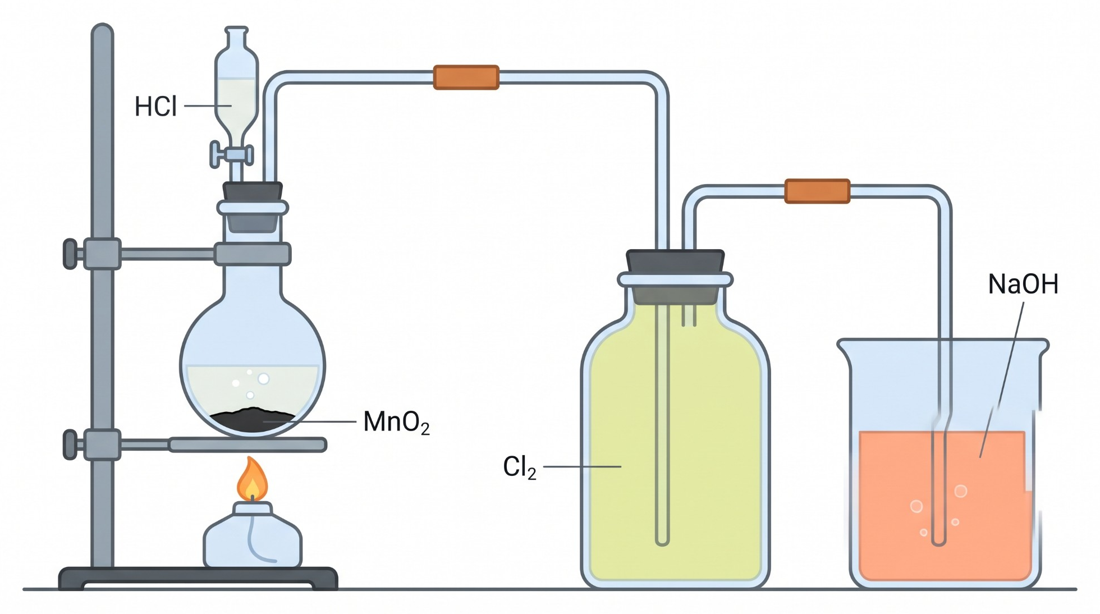
\includegraphics[width=0.86\linewidth]{rasmlar/darslik/d_xlor.png}\end{center}
\noindent A)~\textsl{ortiqcha xlorni yutib, atrof-muhitni zaharlanishdan saqlash}\par
\noindent B)~\textsl{xlorni suvda eritish}\par
\noindent C)~\textsl{xlorni quritish}\par
\noindent D)~\textsl{reaksiyani tezlashtirish}\par
\qsep
\noindent\qn{31.} Laboratoriyada metan olish uchun qaysi moddalar ishlatiladi?
\noindent A)~\textsl{NH\textsubscript{4}Cl + Ca(OH)\textsubscript{2} (qizdirish)}\par
\noindent B)~\textsl{MnO\textsubscript{2} + HCl (kons.)}\par
\noindent C)~\textsl{CH\textsubscript{3}COONa + NaOH (qizdirish)}\par
\noindent D)~\textsl{FeS + HCl}\par
\qsep
\noindent\qn{32.} Raqamlangan (1--4) probirkalarda HCl, Na\textsubscript{2}S, NaOH, Pb(NO\textsubscript{3})\textsubscript{2} eritmalari tartibsiz holda berilgan. Quyidagi kuzatuvlar asosida moddalarni probirka raqami bilan moslang. 2- va 4-probirkalardagi eritmalar aralashtirilganda qora cho`kma tushadi. 1- va 3-probirkalardagi eritmalar aralashtirilganda bir-birini neytrallaydi. 1- va 2-probirkalardagi eritmalar aralashtirilganda oq cho`kma tushadi (mo`l ishqorda eriydi).
\noindent A)~\textsl{1-NaOH, 2-Na\textsubscript{2}S, 3-HCl, 4-Pb(NO\textsubscript{3})\textsubscript{2}}\par
\noindent B)~\textsl{1-HCl, 2-Pb(NO\textsubscript{3})\textsubscript{2}, 3-NaOH, 4-Na\textsubscript{2}S}\par
\noindent C)~\textsl{1-NaOH, 2-Pb(NO\textsubscript{3})\textsubscript{2}, 3-Na\textsubscript{2}S, 4-HCl}\par
\noindent D)~\textsl{1-NaOH, 2-Pb(NO\textsubscript{3})\textsubscript{2}, 3-HCl, 4-Na\textsubscript{2}S   ---}\par
\qsep
\end{multicols}
\medskip
\noindent\setlength{\fboxsep}{0pt}\fbox{\begin{tabular}{p{0.74\linewidth}|p{0.2\linewidth}}
\parbox[t]{0.72\linewidth}{\vspace{3pt}\textbf{Topshiriqlar (33--35) va javob variant (A--F)larini o`zaro to`g`ri moslashtiring.} 0,4 mol/l li NaCl eritmasining 500 ml i inert elektrodlar yordamida 5 A tok kuchi bilan 965 s elektroliz qilindi (eritma hajmi o`zgarmadi deb hisoblang). Ajralgan gazlar aralashmasi yondirilib, hosil bo`lgan gaz 100 g suvda eritildi.
\vspace{3pt}} & \parbox[t]{0.19\linewidth}{\vspace{3pt}A~\textsl{0,9}\\[3pt]
B~\textsl{13}\\[3pt]
C~\textsl{0,3}\\[3pt]
D~\textsl{1,79}\\[3pt]
E~\textsl{26}\\[3pt]
F~\textsl{19,5}}\\ \hline
\parbox[t]{0.72\linewidth}{\vspace{2pt}\textbf{33. Elektrolizdan keyin eritmaning pH ini hisoblang.}\vspace{2pt}} & \\ \hline
\parbox[t]{0.72\linewidth}{\vspace{2pt}\textbf{34. Elektrolizdan keyin eritmada NaCl ning molyar konsentratsiyasini (mol/l) toping.}\vspace{2pt}} & \\ \hline
\parbox[t]{0.72\linewidth}{\vspace{2pt}\textbf{35. Olingan xlorid kislota eritmasining massa ulushini (\%) aniqlang.}\vspace{2pt}} & 
\end{tabular}}
\par\bigskip
\noindent\qn{36.} 25\% li va 5\% li tuz eritmalari massalar nisbati 1 : 1 bo`lgan holda aralashtirildi. Tajriba hajmi 500 ml bo`lgan kolbada o`tkazildi. Hosil bo`lgan eritmaning massa \textbf{ulushini (\%) hisoblang.}
\javob\qsep
\noindent\qn{37.} 4,8 g Mg reaksiyaga kirishdi. Tajriba 40 daqiqa davom etdi. Ajralgan H\textsubscript{2} \textbf{hajmini (l, n.sh.) hisoblang.}
\javob\qsep
\noindent\qn{38.} NaBr va NaI dan iborat 17,8 g aralashma eritilib, mo`l xlor o`tkazildi, eritma bug`latilib quruq qoldiq 8,78 g chiqdi. Tajriba 20 daqiqa davom etdi. Aralashmadagi NaI ning \textbf{massasini (g) toping.}
\javob\qsep
\noindent\qn{39.} Vodorodga nisbatan zichligi 29 bo`lgan alkanning 58 g miqdorining 1/2 qismi yorug`likda xlor bilan monoxlorlandi, hosil bo`lgan xloralkan mo`l KOH ning suvli eritmasi bilan gidrolizlandi. Reagent (KOH) eritmasining massa ulushi 10\% va zichligi 1,3 g/ml; u mo`l miqdorda olingan. Hosil bo`lgan spirtning \textbf{massasini (g) toping.}
\javob\qsep
\noindent\qn{40.} Bir atomli to`yingan noma'lum spirtning 12 g miqdori natriy bilan ta'sirlashganda 2,24 l (n.sh.) vodorod ajraldi. Shu spirtning 1/2 qismi mis(II) oksid bilan oksidlandi, hosil bo`lgan modda mo`l ammiakli kumush oksid eritmasi bilan qizdirildi. Qizdirish 60 daqiqa davom etdi. Ajralgan kumush \textbf{massasini (g) toping.}
\javob\qsep
\par\bigskip\begin{center}\textbf{\fontsize{13}{15}\selectfont YOZMA ISH}\end{center}
\noindent\qn{41.} \textbf{Topshiriqni bajarish jarayonida barcha reaksiya tenglamalarini yozing. Miqdoriy va arifmetik hisoblashlarni (unga asos bo`lgan usul yoki formulani ko`rsatgan holda) uzviy ketma-ketlikda bajaring.}\par\smallskip
\textit{X} -- oksidlanish darajasi +2 bo`lgan metall. \textit{X}(NO\textsubscript{3})\textsubscript{2} tuzining 37,6 g namunasi doimiy massagacha qizdirilganda hosil bo`lgan qattiq qoldiq massasi tuz massasining 42,6\% ini tashkil etdi. Ajralgan gazlar aralashmasi sovitilib, 200 g suvga to`liq yuttirildi; so`ngra qattiq qoldiq hosil bo`lgan eritmada to`liq eritildi (kislota qoldiqsiz sarflandi). Olingan eritma inert elektrodlar yordamida 10 A tok kuchi bilan 3088 s elektroliz qilindi (\textit{X} ning bir qismi eritmada qoldi).\par
\noindent 1)\ Barcha jarayonlarning reaksiya tenglamalarini yozing va tenglashtiring; qoldiq massa ulushidan foydalanib, \textit{X} metallni aniqlang.\par
\noindent 2)\ Qizdirishda ajralgan gazlar tarkibini (mol) toping va ularni suvga yuttirishdan hosil bo`lgan HNO\textsubscript{3} massasini (g) hisoblang.\par
\noindent 3)\ Qoldiq erigandan keyingi eritmada \textit{X}(NO\textsubscript{3})\textsubscript{2} ning massa ulushini (\%) hisoblang. Natijani dastlabki tuz massasi va suv massasi orqali tushuntiring.\par
\noindent 4)\ Elektrolizda katodda ajralgan metall massasini (g) va anodda ajralgan gaz hajmini (l, n.sh.) toping.\par
\noindent 5)\ Elektroliz tugagach eritmadagi \textit{X}(NO\textsubscript{3})\textsubscript{2} va HNO\textsubscript{3} ning massa ulushlarini (\%) aniqlang.\par
\diqqat{Mazkur topshiriq kengaytirilgan javobni talab etib, uning yechilish usuli va shu usul asosidagi barcha hisoblash amallari javoblar varaqasida aks etishi lozim.}\qsep
\noindent\qn{42.} Organik moddalarning xossalarini bilgan holda reaksiya tenglamalarini tugallang va tenglashtiring. 3- va 5-reaksiyalarda hosil bo`lgan asosiy organik mahsulotlarni sistematik nomenklatura bo`yicha nomlang. Hosil bo`lgan organik moddalarning tuzilish formulalarini yozing.\par
\noindent 1)\ CH\textsubscript{3}--CH=CH\textsubscript{2} + HBr $\to$\par
\noindent 2)\ H\textsubscript{2}N--CH\textsubscript{2}--COOH + H\textsubscript{2}N--CH\textsubscript{2}--COOH $\to$\par
\noindent 3)\ 2CH\textsubscript{3}--CH\textsubscript{2}--OH (H\textsubscript{2}SO\textsubscript{4} kons., 140 \textdegree{}C) $\to$\par
\noindent 4)\ C\textsubscript{6}H\textsubscript{5}--NH\textsubscript{2} + Br\textsubscript{2} (suvli eritma) $\to$\par
\noindent 5)\ CH\textsubscript{3}--C$\equiv$CH + 2HCl $\to$\par
\noindent 6)\ H\textsubscript{2}N--CH\textsubscript{2}--COOH + HCl $\to$\par
\noindent 7)\ HCOOCH\textsubscript{3} + NaOH (t) $\to$\par
\diqqat{Mazkur topshiriq kengaytirilgan javobni talab etib, uning yechilish usuli va shu usul asosidagi barcha hisoblash amallari javoblar varaqasida aks etishi lozim.}\qsep
\noindent\qn{43.} \textbf{Topshiriqni bajarish jarayonida barcha reaksiya tenglamalarini yozing. Miqdoriy va arifmetik hisoblashlarni (unga asos bo`lgan usul yoki formulani ko`rsatgan holda) uzviy ketma-ketlikda bajaring.}\par\smallskip
CaCO\textsubscript{3} va MgCO\textsubscript{3} dan iborat 56,8 g aralashma doimiy massagacha qizdirilganda massasi 26,4 g ga kamaydi. Ajralgan gaz 1,05 mol NaOH saqlagan eritmaga yuttirildi (gaz to`liq yutildi), hosil bo`lgan eritmaga mo`l BaCl\textsubscript{2} eritmasi qo`shildi. Qizdirishdan qolgan qattiq qoldiq esa 10\% li xlorid kislotaning stexiometrik miqdorida eritildi. Aralashmaning zichligi 2,3 g/sm\textsuperscript{3} ga teng. Qoldiqning HCl dagi eritmasiga mo`l Na\textsubscript{2}CO\textsubscript{3} eritmasi qo`shilib, hosil bo`lgan cho`kma ajratildi va doimiy massagacha qizdirildi; ajralgan gaz mo`l ohakli suvga yuborildi.\par
\noindent 1)\ Barcha reaksiyalarning tenglamalarini yozing va tenglashtiring. Dastlabki aralashmadagi karbonatlarning massalarini (g) aniqlang.\par
\noindent 2)\ Ajralgan gazning hajmini (l, n.sh.) hisoblang va hosil bo`lgan tuzlar tarkibini (o`rta/nordon) aniqlang.\par
\noindent 3)\ Gaz yutilgandan keyingi eritmadagi tuzlarning massalarini (g) toping. Na\textsubscript{2}CO\textsubscript{3} qo`shilganda hosil bo`lgan cho`kmalarning umumiy massasini (g) hisoblang.\par
\noindent 4)\ BaCl\textsubscript{2} qo`shilganda hosil bo`lgan cho`kma massasini (g) hisoblang. Cho`kma qizdirilganda massa necha gramga kamayadi?\par
\noindent 5)\ Qoldiq erigan eritmaning massasini (g) va undagi tuzlarning massa ulushlarini (\%) toping. Ohakli suvga yuborilganda hosil bo`lgan cho`kma massasini (g) toping.\par
\diqqat{Mazkur topshiriq kengaytirilgan javobni talab etib, uning yechilish usuli va shu usul asosidagi barcha hisoblash amallari javoblar varaqasida aks etishi lozim.}\qsep
\newpage
\noindent\textbf{\fontsize{13}{15}\selectfont 7-variant}\hfill \textbf{Javoblar kaliti}\par\smallskip\hrule\smallskip
\textit{Faqat o`qituvchi uchun.}\par\medskip
\noindent\textbf{1--32-savollar}\par\smallskip
\noindent\begin{tabular}{|c|c|c|c|c|c|c|c|c|c|c|c|c|c|c|c|}\hline
\textbf{1} & \textbf{2} & \textbf{3} & \textbf{4} & \textbf{5} & \textbf{6} & \textbf{7} & \textbf{8} & \textbf{9} & \textbf{10} & \textbf{11} & \textbf{12} & \textbf{13} & \textbf{14} & \textbf{15} & \textbf{16}\\\hline
\textsl{C} & \textsl{D} & \textsl{C} & \textsl{A} & \textsl{B} & \textsl{A} & \textsl{B} & \textsl{B} & \textsl{A} & \textsl{D} & \textsl{B} & \textsl{C} & \textsl{D} & \textsl{A} & \textsl{D} & \textsl{B}\\\hline
\textbf{17} & \textbf{18} & \textbf{19} & \textbf{20} & \textbf{21} & \textbf{22} & \textbf{23} & \textbf{24} & \textbf{25} & \textbf{26} & \textbf{27} & \textbf{28} & \textbf{29} & \textbf{30} & \textbf{31} & \textbf{32}\\\hline
\textsl{B} & \textsl{C} & \textsl{C} & \textsl{B} & \textsl{D} & \textsl{A} & \textsl{D} & \textsl{A} & \textsl{C} & \textsl{C} & \textsl{D} & \textsl{B} & \textsl{A} & \textsl{A} & \textsl{C} & \textsl{D}\\\hline
\end{tabular}\par\medskip
\noindent\textbf{33--35-savollar}\par\smallskip
\noindent\begin{tabular}{|c|c|c|}\hline \textbf{No} & \textbf{Javob} & \textbf{Qiymat}\\\hline
33 & \textsl{B} & 13\\\hline
34 & \textsl{C} & 0,3\\\hline
35 & \textsl{D} & 1,79\\\hline
\end{tabular}\par\medskip
\noindent\textbf{36--40-savollar}\par\smallskip
\noindent\begin{tabular}{|c|c|}\hline \textbf{No} & \textbf{To`g`ri javob}\\\hline
36 & 15\\\hline
37 & 4,48\\\hline
38 & 7,5\\\hline
39 & 37\\\hline
40 & 21,6\\\hline
\end{tabular}\par\medskip
\noindent\textbf{41--43-topshiriqlar: javoblar}\par\smallskip
\noindent\textbf{41-topshiriq.}\par
\noindent 1) 64 $\to$ Cu\par
\noindent 2) 25,2 g\par
\noindent 3) 15,82\%\par
\noindent 4) 10,24 g; 1,79 l\par
\noindent 5) 3,35\%; 8,97\%\par
\noindent\textbf{42-topshiriq.}\par
\noindent 1) CH\textsubscript{3}--CH=CH\textsubscript{2} + HBr $\to$ CH\textsubscript{3}--CHBr--CH\textsubscript{3} (Markovnikov qoidasi)\par
\noindent 2) 2H\textsubscript{2}N--CH\textsubscript{2}--COOH $\to$ H\textsubscript{2}N--CH\textsubscript{2}--CO--NH--CH\textsubscript{2}--COOH + H\textsubscript{2}O\par
\noindent 3) 2CH\textsubscript{3}--CH\textsubscript{2}--OH $\to$ CH\textsubscript{3}--CH\textsubscript{2}--O--CH\textsubscript{2}--CH\textsubscript{3} + H\textsubscript{2}O --- nomi: \textbf{dietil efir (etoksietan)}\par
\noindent 4) C\textsubscript{6}H\textsubscript{5}--NH\textsubscript{2} + 3Br\textsubscript{2} $\to$ C\textsubscript{6}H\textsubscript{2}Br\textsubscript{3}--NH\textsubscript{2}$\downarrow$ + 3HBr\par
\noindent 5) CH\textsubscript{3}--C$\equiv$CH + 2HCl $\to$ CH\textsubscript{3}--CCl\textsubscript{2}--CH\textsubscript{3} --- nomi: \textbf{2,2-dixlorpropan}\par
\noindent 6) H\textsubscript{2}N--CH\textsubscript{2}--COOH + HCl $\to$ [H\textsubscript{3}N--CH\textsubscript{2}--COOH]Cl\par
\noindent 7) HCOOCH\textsubscript{3} + NaOH $\to$ HCOONa + CH\textsubscript{3}OH\par
\noindent\textbf{43-topshiriq.}\par
\noindent 1) 40 g; 16,8 g\par
\noindent 2) 13,44 l\par
\noindent 3) 47,7 g; 12,6 g; 56,8 g\par
\noindent 4) 88,65 g; 26,4 g\par
\noindent 5) 468,4 g; 9,48\%; 4,06\%; 60 g\par
\par\bigskip\noindent\textbf{Mavzular taqsimoti}\par\smallskip
{\small\noindent\begin{longtable}{|c|p{7.2cm}|p{5.4cm}|c|}\hline \textbf{No} & \textbf{Mavzu} & \textbf{Tekshiriladigan ko`nikma} & \textbf{Ball}\\\hline
1 & 8-sinf (metallar va metallmaslar) & Rasm bo`yicha tahlil & 1\\\hline
2 & 8-sinf (vodorod bog`lanish, grafik) & Grafik tahlili & 1\\\hline
3 & Tirkashev I bob; 8-sinf (elektron konfiguratsiya) & Bilim va tushunish & 1\\\hline
4 & 11-sinf 8-bob; Tirkashev \textit{V} bob (elektroliz) & Bilim va tushunish & 1\\\hline
5 & 9-sinf; 11-sinf (pH; neytrallanish) & Hisoblash va masala yechish & 1\\\hline
6 & 9-sinf (metallar, vodorod, suv) & Hisoblash va masala yechish & 1\\\hline
7 & 8-9-sinf (kristallogidratlar) & Hisoblash va masala yechish & 1\\\hline
8 & 9-sinf; 11-sinf (radioaktiv yemirilish) & Hisoblash va masala yechish & 1\\\hline
9 & Tirkashev VI bob (muvozanat, jadval) & Jadval tahlili & 1\\\hline
10 & 9-11-sinf (kimyoviy muvozanat) & Hisoblash va masala yechish & 1\\\hline
11 & 9-sinf (kristallogidratlar) & Hisoblash va masala yechish & 1\\\hline
12 & 8-sinf; Tirkashev VI bob & Jadval tahlili & 1\\\hline
13 & 9-sinf; 11-sinf (reaksiya tezligi; Vant-Goff, massalar ta'siri) & Hisoblash va masala yechish & 1\\\hline
14 & 9-sinf (ishqoriy metallar); Tashev & Bilim va tushunish & 1\\\hline
15 & 9-sinf; Tashev (Fe, Cu, Zn, Cr) & Bilim va tushunish & 1\\\hline
16 & 9-sinf (kislotali oksidlarning ishqor bilan reaksiyasi) & Hisoblash va masala yechish & 1\\\hline
17 & 8-9-sinf (karbonatlar; kislotalar bilan reaksiya) & Hisoblash va masala yechish & 1\\\hline
18 & 9-sinf (xloridlar; sifat reaksiyasi) & Hisoblash va masala yechish & 1\\\hline
19 & 9-11-sinf (gaz hajmi o`zgarishi; parchalanish darajasi) & Hisoblash va masala yechish & 1\\\hline
20 & 10-sinf (mavzuga oid paragraflar); Abdusamatov & Bilim va tushunish & 1\\\hline
21 & 10-sinf (mavzuga oid paragraflar); Abdusamatov & Bilim va tushunish & 1\\\hline
22 & 10-sinf \S{}6, \S{}12, \S{}20, \S{}28 (izomeriya) & Bilim va tushunish & 1\\\hline
23 & 10-sinf (alkenlarni gidrogenlash) & Hisoblash va masala yechish & 1\\\hline
24 & 10-sinf (murakkab efirlarning gidrolizi) & Hisoblash va masala yechish & 1\\\hline
25 & 10-sinf (uglevodlar: kraxmal, glukoza) & Hisoblash va masala yechish & 1\\\hline
26 & 10-sinf (aminlar va anilin xossalari) & Hisoblash va masala yechish & 1\\\hline
27 & 10-sinf (aminokislotalar, peptidlar) & Hisoblash va masala yechish & 1\\\hline
28 & 10-sinf (polimerlar; vinilxlorid olinishi) & Hisoblash va masala yechish & 1\\\hline
29 & 10-sinf (metandan atsetilen, Kucherov, kumush ko`zgu) & Hisoblash va masala yechish & 1\\\hline
30 & 8-sinf (xlor olinishi, 15-rasm) & Rasm bo`yicha tahlil & 1\\\hline
31 & 9--10-sinf (laboratoriya usullari bilan gaz olish) & Bilim va tushunish & 1\\\hline
32 & 9-sinf; 10-sinf (sifat reaksiyalari, ion almashinish) & Bilim va tushunish & 1\\\hline
33--35 & Aralash masala (moslashtirish) & Ko`p bosqichli hisob & 3\\\hline
36--40 & Qisqa javobli masalalar & Hisoblash & 5\\\hline
41--43 & Yozma ish & Usul va hisob (M, A) & 75\\\hline
\end{longtable}}
\end{document}
